\section{Distribución Binomial y Bernoulli}


\subsection{La Distribución Bernoulli y Binomial}


 Si $p$ es la probabilidad de que en un solo ensayo ocurra un evento (llamada la probabilidad de éxito) y $q = 1 - p$ es la
probabilidad de que este evento no ocurra en un solo ensayo (llamada probabilidad de fracaso), entonces la probabilidad de que el evento ocurra exactamente $x$ veces en $N$ ensayos (es decir, que ocurran $x$ éxitos y $N - x$ fracasos) está
dada por
\begin{align}
 \label{eq:2.10.1}
 f(x)=P(X=x)=\comb{N}{x}p^{x}q^{N-x}
\end{align}
donde $x=0,1,...,N.$


 \begin{ejemplo}
  \label{exmp:2.10.1}
  La probabilidad de obtener exactamente dos caras en seis lanzamientos de una moneda es
  \begin{align}
   \comb{6}{2}\left( \dfrac{1}{2} \right)^{2}\left( \dfrac{1}{2} \right)^{6-2}=\dfrac{15}{64}
  \end{align}
empleando \eqref{eq:2.10.1} con $N=6, x=2, p=q=\frac{1}{2}.$
 \end{ejemplo}



\begin{ejemplo}
 \label{exmp:2.10.2}
 Calcule la probabilidad de obtener al menos 4 caras en 6 lanzamientos de una moneda.
\end{ejemplo}

\begin{solucion}
	Usando la distribución binomial con $N=6$, $p=\frac{1}{2}$, $q=\frac{1}{2}$:
	\begin{align}
		P(X \geq 4) &= P(X=4) + P(X=5) + P(X=6) \\
		&= \comb{6}{4}\left(\frac{1}{2}\right)^4\left(\frac{1}{2}\right)^2 + \comb{6}{5}\left(\frac{1}{2}\right)^5\left(\frac{1}{2}\right)^1 + \comb{6}{6}\left(\frac{1}{2}\right)^6 \\
		&= \frac{15}{64} + \frac{6}{64} + \frac{1}{64} = \frac{22}{64} = \frac{11}{32} \approx 0.344
	\end{align}
\end{solucion}



 En lo subsecuente, daremos por hecho que hemos importado los siguientes paquetes:
 \begin{itemize}
  \item \texttt{scipy.stats}
  \item \texttt{numpy} como \texttt{np}
 \end{itemize}


\lstinputlisting[language=Python]{../code/distribuciones-especiales/statsBinom.py}


 \begin{ejemplo}
  \label{exmp:2.10.3}
  Desarrolle $\left( p+q \right)^{4}.$
 \end{ejemplo}


\lstinputlisting[language=Python]{../code/distribuciones-especiales/coefBinom.py}


{Propiedades de la distribución binomial} Supongamos que realizamos $N$ experimentos con probabilidad éxito $p$ y de fracaso $q=1-p.$
\begin{align}
 \label{eq:2.10.2}
 \mu = Np \\
 \label{eq:2.10.3}
 \s^{2}=Npq
\end{align}


\lstinputlisting[language=Python]{../code/distribuciones-especiales/histBinom.py}




 \begin{figure}
 \centering
 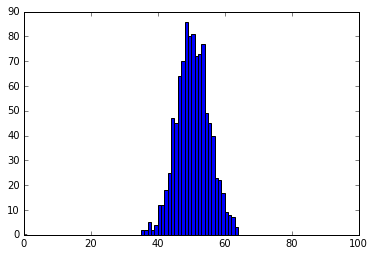
\includegraphics[height=7cm,keepaspectratio=true]{./pe/distBin01.png}
 % distBin01.png: 0x0 pixel, 300dpi, 0.00x0.00 cm, bb=
 \label{fig:2.10.1}
\end{figure}


\section{Distribuciones Geométrica y Binomial Negativa}
\subsection{La Distribución Geométrica}

La distribución geométrica modela el número de ensayos Bernoulli independientes necesarios para obtener el primer éxito. Si cada ensayo tiene probabilidad de éxito $p$ y de fracaso $q=1-p$, entonces la variable aleatoria $X$ que cuenta el número de ensayos hasta obtener el primer éxito (incluyendo el éxito) tiene función de probabilidad
\begin{align}
 \label{eq:2.10.9}
 f(k) = P(X=k) = (1-p)^{k-1}p, \quad k=1,2,3,\dots
\end{align}

Una propiedad fundamental de la distribución geométrica es la \emph{pérdida de memoria}: la probabilidad de obtener un éxito en los siguientes $k$ ensayos no depende del número de fracasos previos. Esto es, si $m,n\geq 1$,
\begin{align}
 P(X > m+n \mid X > m) = P(X > n).
\end{align}

{Propiedades de la distribución geométrica} Si $X$ tiene distribución geométrica con parámetro $p$, entonces
\begin{align}
 \mu_{X} &= \dfrac{1}{p} \\
 \s_{X}^{2} &= \dfrac{1-p}{p^{2}}.
\end{align}

\begin{ejemplo}
 \label{exmp:2.10.13}
 Un vendedor sabe que la probabilidad de cerrar una venta en cada llamada telefónica es $p=0.2$. ¿Cuál es la probabilidad de que necesite realizar exactamente $5$ llamadas para realizar la primera venta? ¿Cuántas llamadas se espera que necesite en promedio?
\end{ejemplo}

\begin{solucion}
	Usando la distribución geométrica con $p=0.2$:
	\begin{align}
		P(X=5) &= (1-0.2)^{5-1}(0.2) = (0.8)^{4}(0.2) \\
		&= 0.4096 \times 0.2 = 0.08192
	\end{align}

	El número esperado de llamadas es
	\begin{align}
		\mu = \dfrac{1}{p} = \dfrac{1}{0.2} = 5.
	\end{align}
\end{solucion}

\begin{ejemplo}
 \label{exmp:2.10.14}
 En un proceso de control de calidad, la probabilidad de que una pieza sea defectuosa es $p=0.1$. ¿Cuál es la probabilidad de que la primera pieza defectuosa aparezca en la tercera inspección?
\end{ejemplo}

\lstinputlisting[language=Python]{../code/distribuciones-especiales/distGeom.py}

\begin{figure}
 \centering
 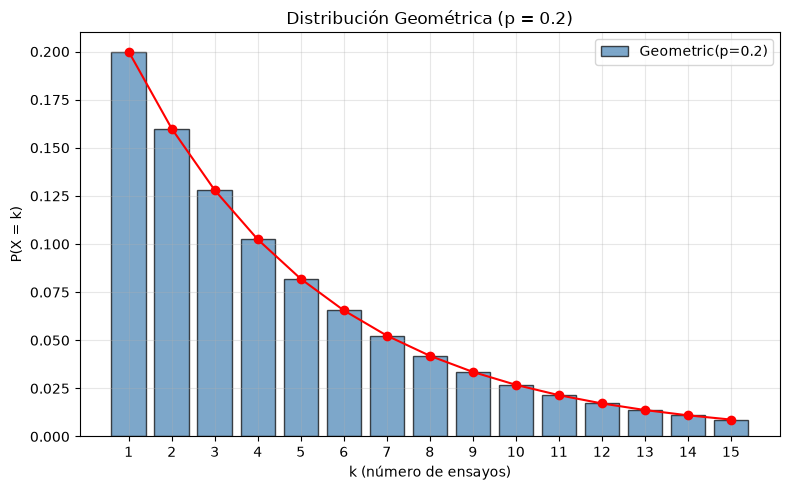
\includegraphics[height=7cm,keepaspectratio=true]{./pe/distGeom.png}
 % distGeom.png: 0x0 pixel, 300dpi, 0.00x0.00 cm, bb=
 \caption{Distribución geométrica con $p=0.2$}
 \label{fig:2.10.7}
\end{figure}



\subsection{La Distribución Binomial Negativa}

La distribución binomial negativa generaliza la geométrica: modela el número de fracasos observados antes de obtener un número predeterminado $r$ de éxitos en una secuencia de ensayos Bernoulli independientes. Su función de probabilidad está dada por
\begin{align}
 \label{eq:2.10.10}
 f(k) = P(X=k) = \binom{k+r-1}{r-1}p^{r}(1-p)^{k}, \quad k=0,1,2,\dots
\end{align}

Observe que cuando $r=1$, la binomial negativa se reduce a la distribución geométrica (contando fracasos antes del primer éxito).

{Propiedades de la distribución binomial negativa} Si $X$ tiene distribución binomial negativa con parámetros $r$ y $p$, entonces
\begin{align}
 \mu_{X} &= \dfrac{r(1-p)}{p} \\
 \s_{X}^{2} &= \dfrac{r(1-p)}{p^{2}}.
\end{align}

\begin{ejemplo}
 \label{exmp:2.10.15}
 Un examen de certificación tiene una tasa de aprobación del $30\%$. ¿Cuál es la probabilidad de que un estudiante repruebe $4$ veces antes de aprobar por tercera vez?
\end{ejemplo}

\begin{solucion}
	En este caso, $r=3$ (número de éxitos) y $p=0.3$. La variable $X$ cuenta el número de fracasos antes del tercer éxito.
	\begin{align}
		P(X=4) &= \binom{4+3-1}{3-1}(0.3)^{3}(0.7)^{4} \\
		&= \binom{6}{2}(0.027)(0.2401) \\
		&= 15 \times 0.027 \times 0.2401 \\
		&\approx 0.0972
	\end{align}
\end{solucion}

\lstinputlisting[language=Python]{../code/distribuciones-especiales/distNegBinom.py}

\begin{figure}
 \centering
 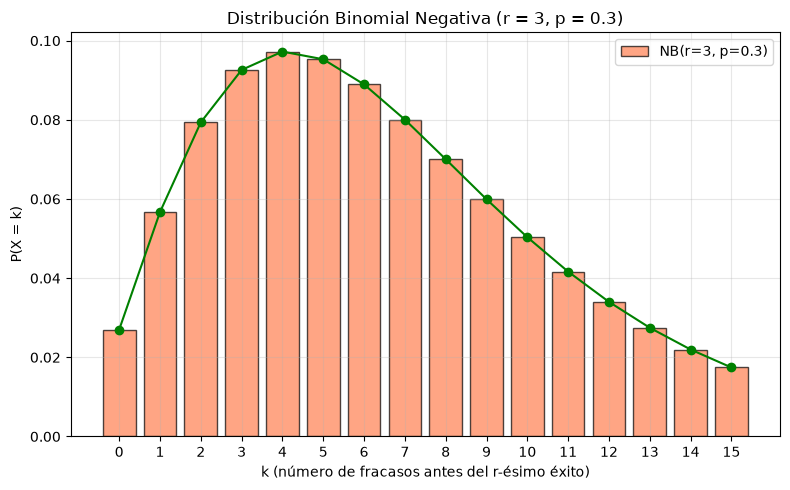
\includegraphics[height=7cm,keepaspectratio=true]{./pe/distNegBinom.png}
 % distNegBinom.png: 0x0 pixel, 300dpi, 0.00x0.00 cm, bb=
 \caption{Distribución binomial negativa con $r=3$, $p=0.3$}
 \label{fig:2.10.8}
\end{figure}



\section{Distribución Hipergeométrica}
\subsection{Muestreo sin reemplazo y fórmulas poblacionales}

La distribución hipergeométrica modela el número de éxitos en $n$ extracciones \emph{sin reemplazo} de una población finita de tamaño $N$ que contiene $K$ éxitos y $N-K$ fracasos. Su función de probabilidad es
\begin{align}
 \label{eq:2.10.11}
 f(k) = P(X=k) = \dfrac{\binom{K}{k}\binom{N-K}{n-k}}{\binom{N}{n}}, \quad \max(0, n-(N-K)) \leq k \leq \min(n, K).
\end{align}

A diferencia de las distribuciones anteriores, los ensayos aquí \emph{no son independientes} porque el muestreo sin reemplazo altera las probabilidades en cada extracción.

{Propiedades de la distribución hipergeométrica} Si $X$ tiene distribución hipergeométrica con parámetros $N$, $K$ y $n$, entonces
\begin{align}
 \mu_{X} &= n\dfrac{K}{N} \\
 \s_{X}^{2} &= n\dfrac{K}{N}\dfrac{N-K}{N}\dfrac{N-n}{N-1}.
\end{align}

El factor $\dfrac{N-n}{N-1}$ se conoce como \emph{factor de corrección por población finita}. Cuando $n \ll N$, este factor tiende a $1$ y la distribución hipergeométrica se aproxima a la binomial con parámetros $n$ y $p=K/N$.

\begin{ejemplo}
 \label{exmp:2.10.16}
 Un lote contiene $20$ piezas, de las cuales $5$ son defectuosas. Si se eligen $4$ piezas al azar sin reemplazo, ¿cuál es la probabilidad de encontrar exactamente $2$ defectuosas?
\end{ejemplo}

\begin{solucion}
	Aquí $N=20$, $K=5$, $n=4$, $k=2$.
	\begin{align}
		P(X=2) &= \dfrac{\binom{5}{2}\binom{15}{2}}{\binom{20}{4}} \\
		&= \dfrac{10 \times 105}{4845} \\
		&= \dfrac{1050}{4845} \approx 0.2167
	\end{align}
\end{solucion}

\begin{ejemplo}
 \label{exmp:2.10.17}
 En una mano de póker de $5$ cartas de una baraja de $52$, ¿cuál es la probabilidad de obtener exactamente $3$ reyes?
\end{ejemplo}

\begin{solucion}
	Aquí $N=52$ (total de cartas), $K=4$ (reyes), $n=5$ (cartas en la mano), $k=3$.
	\begin{align}
		P(X=3) &= \dfrac{\binom{4}{3}\binom{48}{2}}{\binom{52}{5}} \\
		&= \dfrac{4 \times 1128}{2598960} \\
		&= \dfrac{4512}{2598960} \approx 0.00174
	\end{align}
\end{solucion}

\lstinputlisting[language=Python]{../code/distribuciones-especiales/distHyper.py}

\begin{figure}
 \centering
 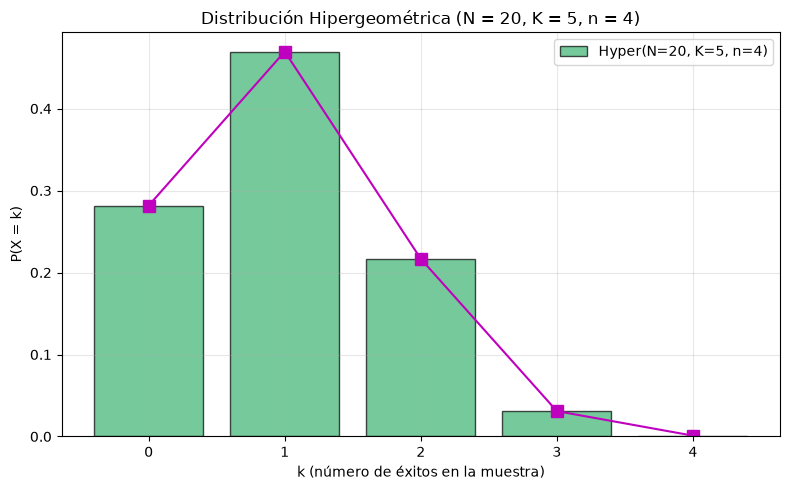
\includegraphics[height=7cm,keepaspectratio=true]{./pe/distHyper.png}
 % distHyper.png: 0x0 pixel, 300dpi, 0.00x0.00 cm, bb=
 \caption{Distribución hipergeométrica con $N=20$, $K=5$, $n=4$}
 \label{fig:2.10.9}
\end{figure}

\begin{observacion}
	La distribución hipergeométrica se reduce a la binomial cuando el muestreo es con reemplazo (o equivalentemente, cuando $N \to \infty$). En la práctica, si $\frac{n}{N} < 0.05$, la aproximación binomial es razonablemente precisa.
\end{observacion}



\section{Distribución de Poisson}
\subsection{La Distribución de Poisson}
{Distribución de Poisson} Diremos que una variable aleatoria \emph{discreta} $X$ tiene distribución de Poisson si su función de probabilidad está dada por:
 \begin{align}
  \label{eq:2.10.7}
  f(n)=\dfrac{\lam^{n}e^{-\lam}}{n!}, \; n=0,1,2,...
 \end{align}


En este caso, $\mu_{X}=\s^{2}=\lam.$


\begin{quote}
 En teoría de probabilidad y estadística, la distribución de Poisson es una distribución de probabilidad discreta que expresa, a partir de una frecuencia de ocurrencia media, la probabilidad de que ocurra un determinado número de eventos durante cierto período de tiempo. Concretamente, se especializa en la probabilidad de ocurrencia de sucesos con probabilidades muy pequeñas, o sucesos raros.
\end{quote}

\href{https://es.wikipedia.org/wiki/Distribuci\%C3\%B3n_de_Poisson}{Wikipedia: Distribución de Poisson}


\begin{ejemplo}
  \label{exmp:2.10.5}
  El número de personas por día que llegan a una sala de urgencia tiene una distribución de Poisson con media 5. Hallar la probabilidad de que cuando mucho lleguen tres por día y la probabilidad de que por lo menos lleguen 8 personas por día.
 \end{ejemplo}

\begin{solucion}
	Usando la distribución de Poisson con $\lambda = 5$:

	\begin{enumerate}
		\item $P(X \leq 3) = \sum_{n=0}^{3} \frac{5^n e^{-5}}{n!}$
		\begin{align}
			&= \frac{5^0 e^{-5}}{0!} + \frac{5^1 e^{-5}}{1!} + \frac{5^2 e^{-5}}{2!} + \frac{5^3 e^{-5}}{3!} \\
			&= e^{-5}(1 + 5 + 12.5 + 20.833) \\
			&= e^{-5} \cdot 39.333 \approx 0.265
		\end{align}

		\item $P(X \geq 8) = 1 - P(X \leq 7)$
		\begin{align}
			&= 1 - \sum_{n=0}^{7} \frac{5^n e^{-5}}{n!} \\
			&\approx 1 - 0.867 = 0.133
		\end{align}
	\end{enumerate}
\end{solucion}




\lstinputlisting[language=Python]{../code/distribuciones-especiales/distPoisson.py}



 \begin{figure}
 \centering
 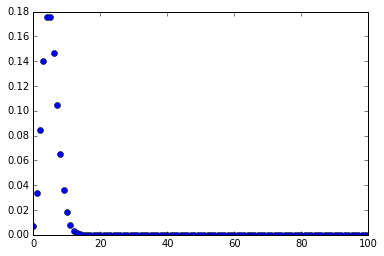
\includegraphics[height=7cm,keepaspectratio=true]{./pe/distPoisson0.png}
 % distPoisson0.png: 0x0 pixel, 300dpi, 0.00x0.00 cm, bb=
 \caption{Distribución de Poisson}
\end{figure}




\begin{figure}
 \centering
 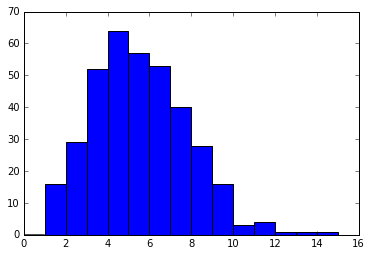
\includegraphics[height=7cm,keepaspectratio=true]{./pe/distPoisson1.png}
 % distPoisson1.png: 0x0 pixel, 300dpi, 0.00x0.00 cm, bb=
 \caption{Histograma de pacientes en sala de urgencias durante un año con media $\lam=5$}
 \label{fig:2.10.6}
\end{figure}



\subsection{Relación entre las Distribuciones Binomiales y de Poisson}

 Si en la función de probabilidad binomial, $N$ es muy grande pero $p \approx 0,$ esto modela un \emph{evento raro}.  En la práctica esto significa $N>>50, Np<<5.$

 En este caso, la distribución Binomial con parámetros $N,p$ se aproxima a una Poisson con parámetro $\lam = Np.$

\lstinputlisting[language=Python]{../code/distribuciones-especiales/relBinomPoisson.py}



 \begin{figure}
 \centering
 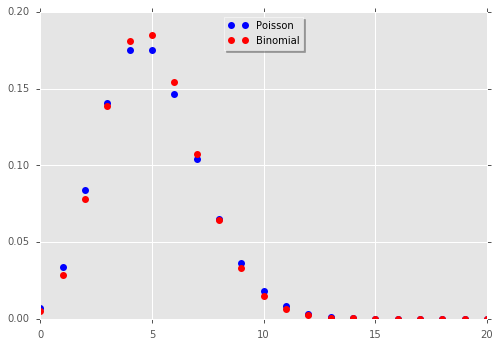
\includegraphics[height=7cm]{./pe/binVsPoi.png}
 % binVsPoi.png: 0x0 pixel, 300dpi, 0.00x0.00 cm, bb=
 \caption{Comparación entre distribuciones Binomial y Poisson para eventos raros.}
\end{figure}



\section{Distribución multinomial}
\subsection{La Distribución multinomial}

 Si los eventos $E_{1},...,E_{k}$ pueden ocurrir con probabilidades $p_{1},...,p_{k}$ respectivamente, entonces la probabilidad de que ocurran $X_{1},...,x_{k}$ veces respectivamente esta dado por la \emph{distribución multinomial}
 \begin{align}
  \label{eq:2.10.8}
  f\left( x_{1},...,x_{k} \right)=
  \dfrac{x_{1}+...+x_{k}}{x_{1}!...x_{k}!}p_{1}^{x_{1}}\cdots p_{k}^{x_{k}}.
 \end{align}



 \begin{ejemplo}
  \label{exmp:2.10.6}
Si un dado se lanza 12 veces, encontrar la probabilidad de obtener cada uno de los números $1,2,3,4,5,6$ exactamente dos veces.
 \end{ejemplo}

\begin{solucion}
	Usando la distribución multinomial con $N=12$, $k=6$, $x_i = 2$ para todo $i$, y $p_i = \frac{1}{6}$ para todo $i$:

	\begin{align}
		P(X_1=2, X_2=2, ..., X_6=2) &= \frac{12!}{2! \cdot 2! \cdot 2! \cdot 2! \cdot 2! \cdot 2!} \left(\frac{1}{6}\right)^2 \cdots \left(\frac{1}{6}\right)^2 \\
		&= \frac{12!}{(2!)^6} \left(\frac{1}{6}\right)^{12} \\
		&= \frac{479001600}{64} \cdot \frac{1}{2176782336} \\
		&\approx 0.00344
	\end{align}
\end{solucion}


\section{Distribución Normal y aproximación continua}
\subsection{Distribución Normal}

 Una de las distribuciones de probabilidad continua más importantes es la \emph{distribución normal}, también llamada \emph{distribución gaussiana,} que se define mediante la función de densidad
 \begin{align}
  \label{eq:2.10.4}
  f_{a,b}(x)=\dfrac{1}{\sqrt{2\pi}}e^{-\frac{1}{2}\frac{(x-a)^{2}}{b^{2}}}
 \end{align}
donde $a,b$ son parámetros específicos para cada v.a. $X.$

{Propiedades de la distribución normal}
 Si la v.a. $X$ tiene la función de densidad dada por \eqref{eq:2.10.4}, con parámetros $a,b$ entonces
 \begin{align}
  a = \mu_{X}\\
  b = \s_{X}
 \end{align}



 Si una variable aleatoria normal $X$ tiene función de densidad
  \begin{align}
  \label{eq:2.10.4a}
  f(x)=\dfrac{1}{\sqrt{2\pi}}e^{-\frac{1}{2}\frac{(x-\mu)^{2}}{\s^{2}}},
  \end{align}
  escribiremos $X\sim N(\mu, \s^{2}).$


{Variable aleatoria normalizada}
 \begin{align}
  \label{eq:2.10.5}
  Z = \dfrac{X-\mu}{\s}\\
  \mu_{Z}=0 \\
  \s_{Z}=1
 \end{align}


{Forma Estándar}
 \begin{align}
  \label{eq:2.10.6}
  f(z)=\dfrac{1}{\sqrt{2\pi}}e^{-\frac{1}{2}z^{2}}
 \end{align}


En este caso, diremos que $Z$ está \emph{normalmente distribuida.}


\lstinputlisting[language=Python]{../code/distribuciones-especiales/distribucionNormal.py}


 \begin{figure}
 \centering
 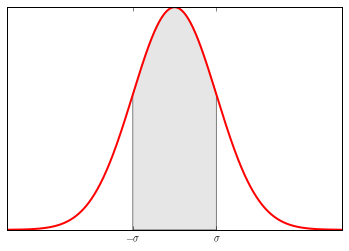
\includegraphics[height=5cm,keepaspectratio=true]{./pe/norm1.png}
 % norm1.png: 0x0 pixel, 300dpi, 0.00x0.00 cm, bb=
 \label{fig:2.10.2}
\end{figure}
\begin{verbatim}
 #(0.682689492137086, 7.579375928402476e-15)
\end{verbatim}


 \begin{figure}
 \centering
 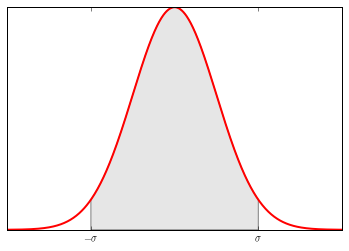
\includegraphics[height=5cm,keepaspectratio=true]{./pe/norm2.png}
 % norm1.png: 0x0 pixel, 300dpi, 0.00x0.00 cm, bb=
 \label{fig:2.10.3}
\end{figure}
\begin{verbatim}
 #(0.9544997361036417, 1.8403548653972355e-11)
\end{verbatim}


 \begin{figure}
 \centering
 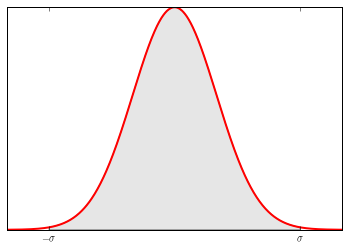
\includegraphics[height=5cm,keepaspectratio=true]{./pe/norm3.png}
 % norm1.png: 0x0 pixel, 300dpi, 0.00x0.00 cm, bb=
 \label{fig:2.10.4}
\end{figure}
\begin{verbatim}
 #(0.9973002039367399, 1.1072256503105314e-14)
\end{verbatim}


 \begin{figure}
 \centering
 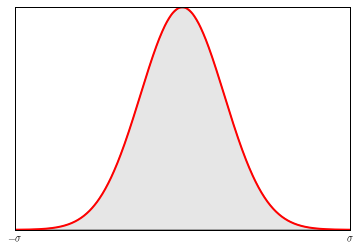
\includegraphics[height=5cm,keepaspectratio=true]{./pe/norm4.png}
 % norm1.png: 0x0 pixel, 300dpi, 0.00x0.00 cm, bb=
 \label{fig:2.10.5}
\end{figure}
\begin{verbatim}
 #(0.9999366575163339, 4.838904125482879e-12)
\end{verbatim}


\lstinputlisting[language=Python]{../code/distribuciones-especiales/normalCDF.py}
\begin{center}
 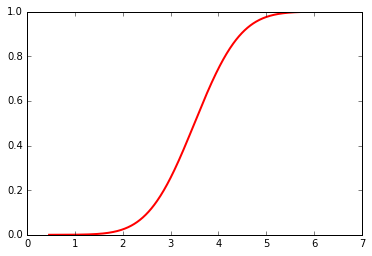
\includegraphics[height=5cm,keepaspectratio=true]{./pe/normCDF.png}
 % normCDF.png: 0x0 pixel, 300dpi, 0.00x0.00 cm, bb=
\end{center}



\subsection{Relación entre las distribuciones binomial y normal}

 Si $N\sim \infty, p,q>>0,$ y $X$ es un distribución binomial con parámetros $N,p$ entonces
 \begin{align}
  \dfrac{X-Np}{\sqrt{Npq}} \sim N(0,1).
 \end{align}



 \begin{ejemplo}
  \label{exmp:2.10.4}
  Consideremos el experimento de lanzar 16 veces una moneda. Repitamos 1,000,000 dicho experimento. Compruebe que dicho experimento se puede modelar por una variable aleatoria con distribución $N(\mu=8,\sigma^{2}=4)$
 \end{ejemplo}


\lstinputlisting[language=Python]{../code/distribuciones-especiales/relBinomNormal.py}
\begin{center}
 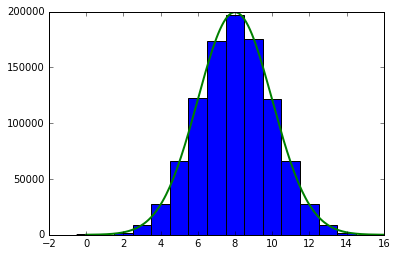
\includegraphics[height=5cm]{./pe/relBinNorm.png}
 % relBinNorm.png: 0x0 pixel, 300dpi, 0.00x0.00 cm, bb=
\end{center}


\subsection{Problemas Resueltos}
{Percentil}
 Diremos que $x=P_{q}$ es el percentil $q, \; 0\leq q \leq 100$ de la distribución $F(x)$ si $F(P_{q})=q\%.$  En el caso de que $q$ sea un valor realizable de $F(x),$ podemos \emph{``despejar''}
 \begin{align}
  P_{q}=F^{-1}\left( \dfrac{q}{100} \right).
 \end{align}
 A tal función se le llama \emph{distribución inversa.}


{Cuartiles}
 En la literatura se definen conceptos similares. Por ejemplo, el primer \emph{cuartil} corresponde al percentil $25;$ el segundo cuartil al percentil $50;$ y así sucesivamente.

{Combinaciones}
 \begin{ejemplo}
  \label{exmp:2.10.7}
  Encuentre
  \begin{enumerate}
   \item $5!$
   \item $\comb{8}{3}$
  \end{enumerate}
  utilizando \texttt{Python.}
 \end{ejemplo}


\lstinputlisting[language=Python]{../code/distribuciones-especiales/combinaciones.py}




{Distribución Binomial}
 \begin{ejemplo}
  \label{exmp:2.10.8}
  Supóngase que $15\%$ de la población es zurda. Encontrar la probabilidad de que en un grupo de 50 individuos haya:
  \begin{enumerate}
   \item cuando mucho 10 zurdos;
   \item por lo menos 5 zurdos;
   \item entre 3 y 6 zurdos;
   \item exactamente 5 zurdos.
  \end{enumerate}

 \end{ejemplo}


\lstinputlisting[language=Python]{../code/distribuciones-especiales/solvedBinom.py}



{Distribución Normal}
 \begin{ejemplo}
  \label{exmp:2.10.9}
  En un examen final de matemáticas, la media fue 72 y la desviación estándar fue 15. Determinar las puntuaciones estándar de los estudiantes que obtuvieron:
  \begin{enumerate}
   \item $60$;
   \item $93$;
   \item $72$.
  \end{enumerate}

 \end{ejemplo}



 \begin{ejemplo}
   \label{exmp:2.10.10}
   Con los datos del problema \ref{exmp:2.10.9}, encontrar las calificaciones que corresponden a las siguientes puntuaciones estándar:
  \begin{enumerate}
   \item $-1$;
   \item $1.6$.
  \end{enumerate}

 \end{ejemplo}



 \begin{ejemplo}
  \label{exmp:2.10.11}
  Supóngase que la cantidad de juegos en que participan los beisbolistas de la liga mayor durante su carrera se distribuye normalmente con media de $1500$ juegos y desviación estándar $350$ juegos. Emplear \texttt{Python} para responder las siguientes preguntas:
  \begin{enumerate}
   \item ¿Qué porcentaje participa en menos de 750 juegos?;
   \item ¿qué porcentaje participa en más de 2000 juegos?;
   \item encontrar el \emph{percentil} $90$ de la cantidad de juegos en los que participan en su carrera.
  \end{enumerate}

 \end{ejemplo}


\lstinputlisting[language=Python]{../code/distribuciones-especiales/solvedNorm.py}


{Eventos raros}
\begin{ejemplo}
\label{exmp:2.10.12}
  Si la probabilidad de que un individuo tenga una reacción adversa por la inyección de determinado suero es $0.001,$ determinar la probabilidad de que de 2000 individuos:
 \begin{enumerate}
  \item exactamente 3;
  \item más de 2
 \end{enumerate}
sufran una reacción adversa.
\end{ejemplo}


\lstinputlisting[language=Python]{../code/distribuciones-especiales/eventosRaros.py}



\section{Distribuciones discretas en ciencia de datos}
\subsection{Distribuciones discretas y su relación con ciencia de datos}

Las distribuciones discretas estudiadas en este capítulo no son solo objetos teóricos: son herramientas fundamentales en el análisis y modelado de datos. A continuación se resumen sus aplicaciones más comunes en ciencia de datos.

\begin{itemize}
 \item \textbf{Distribución binomial:} Se utiliza en pruebas A/B para determinar si existe una diferencia estadísticamente significativa entre dos tasas de conversión. También es la base de muchos modelos de clasificación binaria.

 \item \textbf{Distribución de Poisson:} Modela la frecuencia de eventos raros en un intervalo fijo, como el número de visitas a una página web por minuto, las llamadas a un centro de atención por hora, o los defectos por unidad de producción. Es ampliamente usada en análisis de tráfico y detección de anomalías.

 \item \textbf{Distribución geométrica:} Modela el número de ensayos hasta el primer éxito. En ciencia de datos se aplica en análisis de supervivencia (tiempo hasta la primera conversión), modelado de churn y en el diseño de estrategias de retención.

 \item \textbf{Distribución binomial negativa:} Es una extensión de Poisson que permite modelar datos de conteo con \emph{sobredispersión} (varianza mayor que la media). Es frecuente en datos reales donde la variabilidad excede la predicha por Poisson, por ejemplo en el número de transacciones por cliente o el número de clics por usuario.

 \item \textbf{Distribución hipergeométrica:} Se emplea cuando se trabaja con muestras sin reemplazo de poblaciones finitas, como en auditorías de calidad, muestreo de encuestas, o en pruebas estadísticas exactas como la prueba exacta de Fisher.
\end{itemize}

\begin{ejemplo}
 \label{exmp:2.10.18}
 Se quiere analizar el número de clicks que reciben $100$ anuncios publicitarios en una hora. Los datos observados tienen media $\bar{x}=4.2$ y varianza $s^{2}=8.7$. ¿Es razonable modelar estos datos con una distribución de Poisson?
\end{ejemplo}

\begin{solucion}
	En una distribución de Poisson, la media y la varianza son iguales: $\mu = \sigma^{2} = \lambda$. Como en este caso $s^{2} = 8.7 \gg \bar{x} = 4.2$, los datos presentan \emph{sobredispersión}. Por lo tanto, una distribución de Poisson \emph{no} es adecuada. En su lugar, se recomienda usar una distribución binomial negativa, que permite modelar esta variabilidad adicional.
\end{solucion}

\lstinputlisting[language=Python]{../code/distribuciones-especiales/distDataScience.py}

\begin{figure}
 \centering
 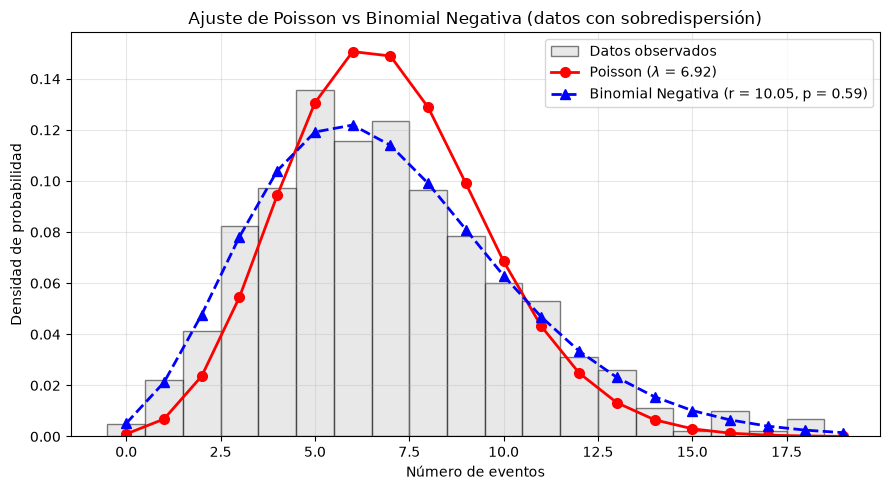
\includegraphics[height=7cm,keepaspectratio=true]{./pe/distDataScience.png}
 % distDataScience.png: 0x0 pixel, 300dpi, 0.00x0.00 cm, bb=
 \caption{Comparación de ajuste de Poisson vs. Binomial Negativa para datos con sobredispersión}
 \label{fig:2.10.10}
\end{figure}

\begin{observacion}
	En la práctica, la elección de la distribución depende tanto de la naturaleza del fenómeno modelado como de las propiedades estadísticas de los datos observados. Herramientas como la función de verosimilitud, el criterio de información de Akaike (AIC) o validación cruzada permiten comparar distintos modelos y elegir el más apropiado.
\end{observacion}


